\documentclass[border=2mm]{standalone}
\usepackage{tikz}
\usepackage[scaled=0.95]{helvet}
\renewcommand{\familydefault}{\sfdefault}
\begin{document}
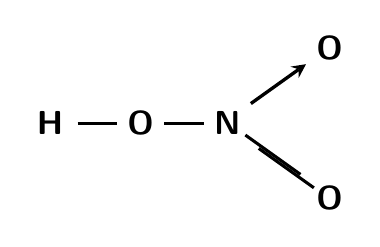
\begin{tikzpicture}[line width=1.1pt]
  \node at (0,0) {\large \textbf{H}};
  \draw (0.35,0) -- (0.85,0);
  \node at (1.15,0) {\large \textbf{O}};
  \draw (1.45,0) -- (1.95,0);
  \node at (2.25,0) {\large \textbf{N}};
  
  % arrow up-right to O
  \draw[->, >=stealth, line width=1.2pt] (2.55, 0.25) -- (3.25, 0.75);
  \node at (3.55, 0.95) {\large \textbf{O}};
  
  % double bond down-right to O
  \draw[line width=1.1pt] (2.48, -0.15) -- (3.18, -0.65);
  \draw[line width=1.1pt] (2.65, -0.32) -- (3.35, -0.82);
  \node at (3.55, -0.95) {\large \textbf{O}};
\end{tikzpicture}
\end{document}
